\graphicspath{{../images/algorithm/}}
\chapter{Экспериментальные результаты}
%\section{Поиск и обработка исходных данных для оценки работы алгоритма}
%\cite{asedb2001}

%\cite{kortemme_alascan_datasets}
%\cite{sdr1}
%\todo{глава не готова}
\section{Пример работы итеративного алгоритма выбора протяженных регионов}
Для оценки корректности работы алгоритма на каждом из этапов проводился визуальный контроль выбираемых аминокислот с использованием средств визуализации приложения PyMol ~\cite{pymol}.

Далее приведены несколько рисунков с L и H цепями антитела (структура с идентификатором 2OSL, с исключенными молекулами воды) с разных ракурсов, на которых выделены разными цветами аминокислоты, добавляемые к региону для аланинового сканирования на разных этапах:
\begin{itemize}

\item желтым цветом изображена L-цепь, на ней голубым цветом выделены аминокислоты, содержащие атомы, которые попали в начальное отобранное множество треугольников выпуклой оболочки;

\item синим цветом выделены аминокислоты, атомы которых попали в выделенную область на этапе поиска карманов;

\item красным цветом выделены участки цепочки, которые были добавлены в результате добавления петель, частично попавших в выделенный регион на одном из предыдущих этапов.
\end{itemize}

\begin{figure}
%\resizebox{0.8\textwidth}{!}{
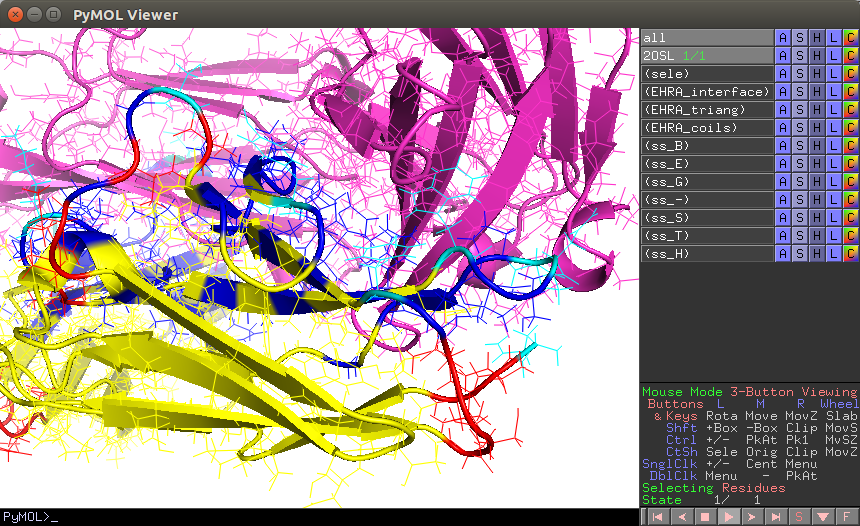
\includegraphics[width=0.85\linewidth]{loops1.png}
%}

\caption{\small{Структура 2OSL: красным цветом показаны добавляемые к региону, определяющему специфичность, фрагменты петель; синим цветом показан сам регион}}
\label{fig:loops1}
\end{figure}


%\begin{figure}
%\resizebox{0.8\textwidth}{!}{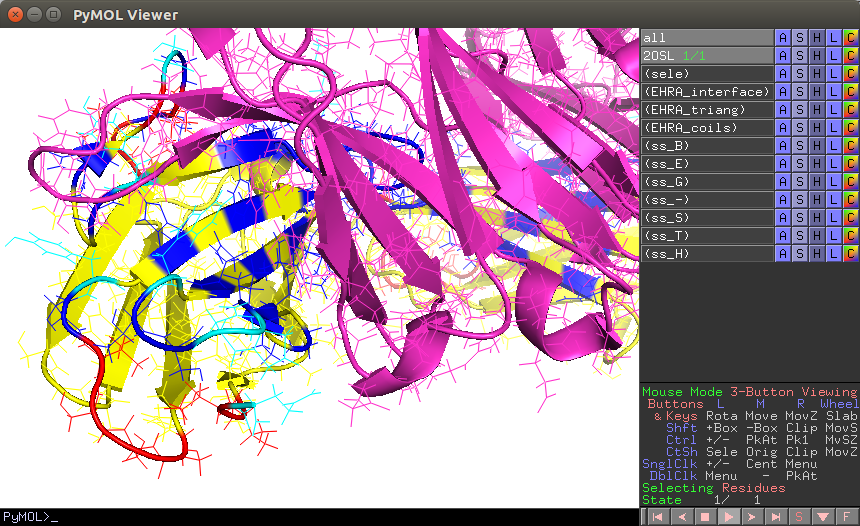
\includegraphics[width=\linewidth]{loops2.png}
%}

%\caption{\small{[Computation of tunnels in protein molecules using
%Delaunay triangulation, P.Medek, et al., 2007]
% }}
%\label{fig:loops2}
%\end{figure}



%На последнем из приведенных скриншотов в нижней части изображения видна петля, которая удалена от интерфейса взаимодействия, но при этом один из атомов ее аминокислот по удачному стечению обстоятельств попал в множество отобранных треугольников выпуклой оболочки, за счет чего петля попала целиком.

%\todo{И это наводит на мысль о том, что изначальный выбор аминокислот не так хорош. Возможно, стоит использовать граф Габриэля? }


%\begin{figure}
%\resizebox{0.8\textwidth}{!}{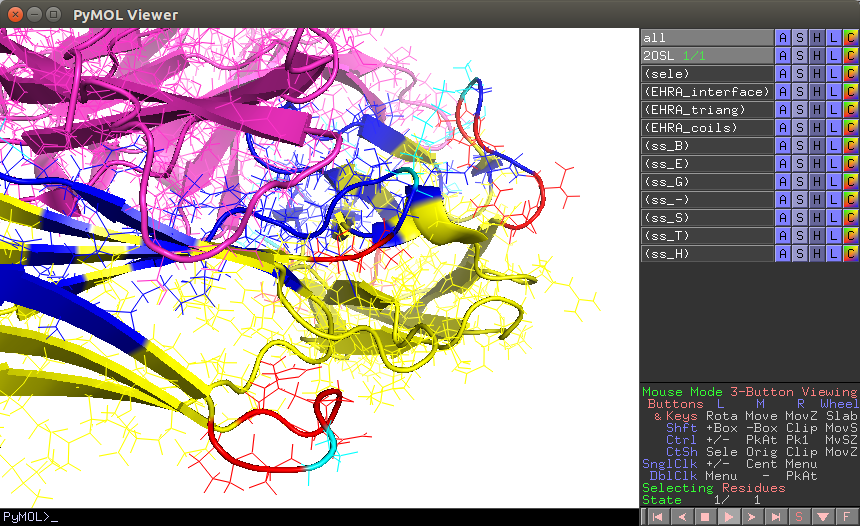
\includegraphics[width=\linewidth]{loops3.png}
%}

%\caption{\small{Структура 2OSL: красным цветом показаны добавляемые к региону, определяющему специфичность, фрагменты петель; синим цветом показан сам регион
% }}
%\label{fig:loops3}
%\end{figure}



%Посередине петля полностью желтая - но это из-за способа, которым добавлялись карманы.


\begin{figure}
%\resizebox{0.8\textwidth}{!}{
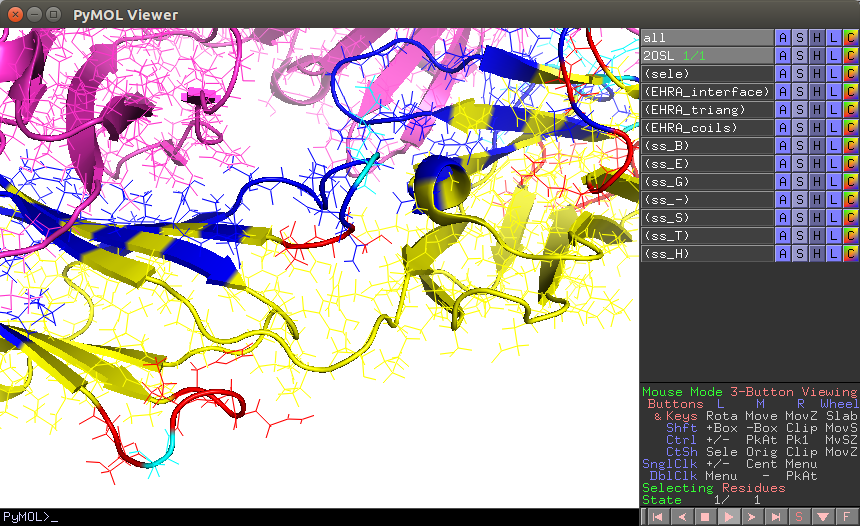
\includegraphics[width=0.85\linewidth]{loops4.png}
%}

\caption{\small{Структура 2OSL: красным цветом показаны добавляемые к региону, определяющему специфичность, фрагменты петель; синим цветом показан сам регион
 }}
\label{fig:loops4}
\end{figure}


\newpage
%\section{Протокол аланинового сканирования}
% http://www.bakerlab.org/system/files/kortemme04B.pdf
% - картинка отсюда с страницы 3
%\todo{-нужна картинка про rosetta alascan protocol }

%В работе \cite{kortemme2002} показано, что (сказать про функцию энергии для компьютерного моделирования аланинового сканирования)

%\todo{-описание того, в какой части предполагается использовать модиф регионы}
%\vspace{10cm}


\newpage
\section{Пример работы на структурах с известными результатами  экспериментального аланинового сканирования}
%Уже обработанные данные есть здесь: \cite{kortemme_alascan_datasets}

%Картинка \cite{benchmark_img} но я не уверена, можно ли ее приводить без разрешения

%\todo{- картинка с схемой работы скрипта}

%\todo{- красивая табличка, с процентом аминокислот в цепочке, попавших в регион, а также попавшими и не попавшими хотспотами.}
%Описание таблички (нужно для корректного вывода в скрипте)
% 1. идентификатор файла pdb
% 2. мутируемая цепь
% 3. цепь\ лиганд, взаимодействие с которым оценивается
% 4. длина цепочки, длина региона, число замаскированных амк
% 5.
%\\

%\todo{-написать скрипт, который для данного pdb и пары цепочек проводит ala-scan по всем позициям и сравнивает методы, которые используются для фильтрации аминокислот.}

%\todo{сделать табличку по данным asedb и bid, и для того, что нет (хотспоты искать с помощью протокола аланинового сканирования, в табличке рисовать циферки). если есть амк, которые не нашлись,}
%\vspace{10cm}

Определим термины, с помощью которых мы будем оценивать качество работы метода. Назовем энергетически значимые аминокислоты  положительными, а аминокислоты, которые значимыми не являются -- отрицательными.

Истинно-положительное
наблюдение (также будем обозначать его TP - сокращение от true positive) --
наблюдение, правильно определенное как положительное. В нашем случае истинно-положительные наблюдения -- это энергетически значимые аминокислоты, которые попали в регион в результате работы алгоритма.

Ложно-положительное наблюдение (FP, или false positive) -- наблюдение, не правильно
определенное как положительное. В нашем случае ложно-положительные наблюдения -- аминокислоты, которые попали в выбранный регион и которые энергетически значимыми не являются.

Истинно-отрицательное наблюдение (TN, или true negative) -- наблюдение, правильно определенное как отрицательное. В нашем случае аминокислоты, которые не были выбраны алгоритмом и которые энергетически значимыми не являются.

Ложно-отрицательное наблюдение (FN, или false negative) -- наблюдение, не правильно определенное как отрицательное. В нашем случае это аминокислоты, которые являются энергетически значимыми но не были выбраны алгоритмом.

Обозначим все положительные наблюдения P, а  все отрицательные -- N.

Отношение числа истинно-положительных наблюдений TP к числу истинных наблюдений P, то есть долю энергетически значимых аминокислот, которые были выявлены алгоритмом, по отношению к всем энергетически значимым аминокислотам цепочки, будем обозначать TPR. 


Был проведен поиск регионов для структур, содержащихся в наборе данных для бенчмаркинга Kortemme \& Baker \cite{kortemme_alascan_datasets} (без учета воды, изначальный набор атомов выпуклой оболочки определялся со значением отсечки по расстоянию 5 \AA{}). Результаты работы скрипта для двухцепочечных структур приведены в таблице \ref{tab:comparison}.
\begin{table}[h]
\begin{center}
\caption{Результат поиска регионов, определяющих специфичность, на структурах набора данных Kortemme \& Baker (две цепочки) }
\label{tab:comparison}
\begin{tabular}{|c|c|c|c|c|c|c|c|c|}
\hline
 PDB & chain & P+N & TP+FP & TP & TP+FN & FN & TPR & ACC \\
 \hline
  1 & 2 & 3 & 4 & 5 & 6 & 7 & 8 & 9 \\
 \hline
1A22 & A & 180 & 85 & 29 & 29 & 0 & 1.0000 & 0.6889\\
1A22 & B & 192 & 166 & 36 & 36 & 0 & 1.0000 & 0.3229\\
1BXI & A & 83 & 67 & 29 & 30 & 1 & 0.9667 & 0.5301\\
1DFJ & I & 456 & 215 & 11 & 14 & 3 & 0.7857 & 0.5461\\
1F47 & A & 17 & 17 & 9 & 9 & 0 & 1.0000 & 0.5294\\
1FC2 & C & 45 & 41 & 3 & 3 & 0 & 1.0000 & 0.1556\\
2PTC & I & 58 & 52 & 1 & 1 & 0 & 1.0000 & 0.1207\\
\hline
\end{tabular}
\end{center}
\end{table}
\\[10pt]
Расшифровка: 
\begin{itemize}
\item графы 1 и 2 - имя файла со структурой в Protein Data Bank и цепочки, на которой расположены энергетически значимые аминокислоты;
\item 3 графа - число аминокислот в цепочке;
\item 4 графа = число аминокислот, выбранных алгоритмом поиска регионов;
\item 5 графа - число аминокислот-хотспотов на цепочке по данным из базы данных;
\item 6 графа - число аминокислот-хотспотов, находящихся в выбранном алгоритмом регионе;
\item 7 графа - число аминокислот-хотспотов, которые есть в базе, но которые не попали в выбранный протяженный регион;
\item следующие графы - рассчитанные характеристики.
\end{itemize}

На рисунке \ref{fig:1BXI} приведена цепочка A структуры 1BXI, с выделенными на ней областями. Красным цветом показаны элементы вторичной структуры, попавшие в выделенный регион, желтым цветом изображена аминокислота, которая является энергетически значимой, но которая в выделенный регион не попала.

\begin{figure}
%\resizebox{0.8\textwidth}{!}{
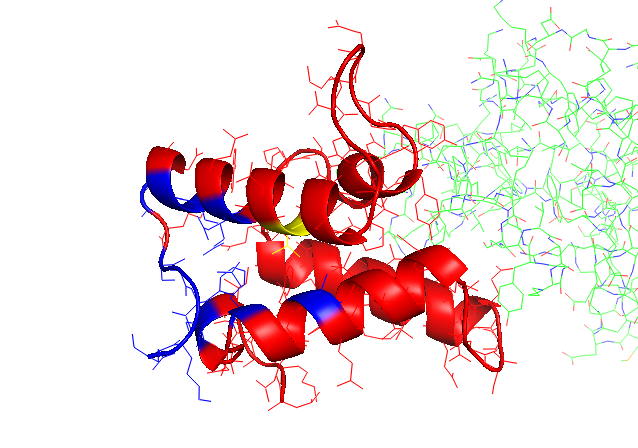
\includegraphics[width=0.85\linewidth]{1BXI.png}
%}
\caption{\small{Структура 1BXI
 }}
\label{fig:1BXI}

\end{figure}

Для второй структуры, у которой в выделенный протяженный регион попали не все энергетически значимые аминокислоты (1DFJ), снимок экрана приведен на рисунке \ref{fig:1DFJ}. Такой результат объясняется тем, что интерфейс взаимодействия расположен в кармане, а также текущим способом поиска карманов, используемым в алгоритме.


\begin{figure}[h]
%\resizebox{0.8\textwidth}{!}{
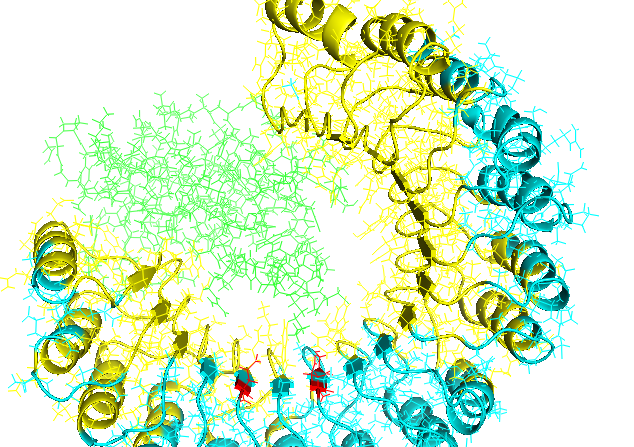
\includegraphics[width=\linewidth]{1DFJ.png}
%}

\caption{\small{Структура с идентификатором  1DFJ в Protein Data Bank. Энергетически значимые аминокислоты, не попавшие в регион, определяющий специфичность, показаны красным цветом, выделенный регион - желтым цветом, остальная часть цепочки показана голубым цветом.
 }}
\label{fig:1DFJ}
\end{figure}



В остальных случаях для двух цепочек энергетически горячие аминокислоты нашлись все (TPR=1). Маленькие значения точности (ACC) можно объяснить тем, что для начального выбора атомных центров-вершин выпуклой оболочки берется фиксированная отсечка по расстоянию, что может приводить в отдельных случаях к выбору в состав региона для сканирования большей части цепочки или всей цепочки.

Для сравнения была построена таблица с результатами выбора аминокислот с ограничением по расстоянию от второй цепочки (таблица \ref{tab:comparison2}). Несмотря на то, что число позиций, выбираемых при таком способе, меньше, частота ,,угадывания'' большего числа энергетически значимых аминокислот выше.
\begin{table}[h]
\begin{center}
\caption{Результат выбора аминокислот с отсечкой по расстоянию (5 \AA{}), на структурах набора данных Kortemme \& Baker (две цепочки) }
\label{tab:comparison2}
\begin{tabular}{|c|c|c|c|c|c|c|c|c|}
\hline
 PDB & chain & P+N & TP+FP & TP & TP+FN & FN & TPR & ACC \\
 \hline
  1 & 2 & 3 & 4 & 5 & 6 & 7 & 8 & 9 \\
 \hline
1A22 & A & 180 & 33 & 24 & 29 & 5 & 0.8276 & 0.9222\\
1A22 & B & 192 & 33 & 27 & 36 & 9 & 0.7500 & 0.9219\\
1BXI & A & 83 & 23 & 16 & 30 & 14 & 0.5333 & 0.7470\\
1DFJ & I & 456 & 39 & 13 & 14 & 1 & 0.9286 & 0.9408\\
1F47 & A & 17 & 9 & 8 & 9 & 1 & 0.8889 & 0.8824\\
1FC2 & C & 45 & 16 & 3 & 3 & 0 & 1.0000 & 0.7111\\
2PTC & I & 58 & 14 & 1 & 1 & 0 & 1.0000 & 0.7759\\
\hline
\end{tabular}
\end{center}
\end{table}


С PDB-файлами, которые содержали более 2 цепочек, была проведена аналогичная процедура с усложнением: энергетически значимые аминокислоты сгруппированы по цепочкам, для каждой из этих цепочек парная цепочка, относительно которой выбирался регион, была определена как одна из оставшихся цепочек. Результаты работы для пар цепочек, некоторые из атомов которых удалены друг от друга не более, чем на 5 \AA{}, приведены в таблице \ref{tab:multichain}-\ref{tab:multichain2} (расшифровка граф аналогична расшифровке в предыдущем случае).
\begin{table}
\begin{center}
\caption{Результат поиска регионов, определяющих специфичность, на структурах набора данных Kortemme \& Baker (больше 2 цепочек в структуре)}
\label{tab:multichain}
\resizebox{\linewidth}{!}{
\begin{tabular}{|c|c|c|c|c|c|c|c|c|c|c|}
\hline
pdb & chain1 & chain2 & P+N & TP+FP & TP+FN & TP & TPR & ACC \\
\hline
1 & 2 & 3 & 4 & 5 & 6 & 7 & 8 & 9 \\
\hline
1CBW & D & B & 58 & 52 & 8 & 8 & 1.0000 & 0.2414\\
1CBW & D & C & 58 & 51 & 8 & 8 & 1.0000 & 0.2586\\
1CBW & D & G & 58 & 53 & 8 & 8 & 1.0000 & 0.2241\\
1CBW & D & H & 58 & 28 & 8 & 1 & 0.1250 & 0.4138\\
1CBW & D & I & 58 & 46 & 8 & 7 & 0.8750 & 0.3103\\
\hline
1DAN & U & L & 116 & 112 & 23 & 23 & 1.0000 & 0.2328\\
1DAN & U & H & 116 & 84 & 23 & 18 & 0.7826 & 0.3879\\
1DAN & U & T & 116 & 96 & 23 & 19 & 0.8261 & 0.3017\\
1DAN & T & L & 75 & 75 & 20 & 20 & 1.0000 & 0.2667\\
1DAN & T & H & 75 & 58 & 20 & 13 & 0.6500 & 0.3067\\
1DAN & T & U & 75 & 75 & 20 & 20 & 1.0000 & 0.2667\\
\hline
1JRH & I & L & 95 & 80 & 12 & 12 & 1.0000 & 0.2842\\
1JRH & I & H & 95 & 81 & 12 & 12 & 1.0000 & 0.2737\\
1JRH & H & L & 171 & 135 & 11 & 9 & 0.8182 & 0.2515\\
1JRH & H & I & 171 & 144 & 11 & 10 & 0.9091 & 0.2105\\
1JRH & L & H & 167 & 127 & 8 & 8 & 1.0000 & 0.2874\\
1JRH & L & I & 167 & 90 & 8 & 8 & 1.0000 & 0.5090\\
\hline
1GC1 & C & G & 181 & 163 & 49 & 49 & 1.0000 & 0.3702\\
\hline
1AHW & C & A & 200 & 168 & 8 & 8 & 1.0000 & 0.2000\\
1AHW & C & B & 200 & 166 & 8 & 8 & 1.0000 & 0.2100\\
\hline
\end{tabular}
}
\end{center}
\end{table}

\begin{table}
\begin{center}
\caption{Результат поиска регионов, определяющих специфичность, на структурах набора данных Kortemme \& Baker (больше 2 цепочек в структуре -- продолжение)}
\label{tab:multichain2}
\resizebox{\linewidth}{!}{
\begin{tabular}{|c|c|c|c|c|c|c|c|c|c|c|}
\hline
pdb & chain1 & chain2 & P+N & TP+FP & TP+FN & TP & TPR & ACC \\
\hline
1 & 2 & 3 & 4 & 5 & 6 & 7 & 8 & 9 \\
\hline
1NMB & H & N & 113 & 109 & 1 & 1 & 1.0000 & 0.0442\\
1NMB & H & L & 113 & 89 & 1 & 1 & 1.0000 & 0.2212\\
\hline
1FCC & C & A & 56 & 56 & 8 & 8 & 1.0000 & 0.1429\\
\hline
1BRS & A & B & 108 & 60 & 8 & 6 & 0.7500 & 0.4815\\
1BRS & A & D & 108 & 85 & 8 & 8 & 1.0000 & 0.2870\\
\hline
3HFM & Y & L & 129 & 93 & 13 & 13 & 1.0000 & 0.3798\\
3HFM & H & L & 215 & 176 & 8 & 8 & 1.0000 & 0.2186\\
3HFM & H & Y & 215 & 125 & 8 & 8 & 1.0000 & 0.4558\\
3HFM & L & Y & 214 & 95 & 5 & 5 & 1.0000 & 0.5794\\
\hline
1DN2 & A & B & 215 & 172 & 3 & 3 & 1.0000 & 0.2140\\
1DN2 & E & A & 14 & 14 & 2 & 2 & 1.0000 & 0.1429\\
\hline
1A4Y & A & B & 460 & 241 & 14 & 14 & 1.0000 & 0.5065\\
1A4Y & A & D & 460 & 305 & 14 & 11 & 0.7857 & 0.3543\\
1A4Y & A & E & 460 & 246 & 14 & 9 & 0.6429 & 0.4739\\
1A4Y & B & A & 123 & 104 & 14 & 14 & 1.0000 & 0.2683\\
\hline
1VFB & A & B & 107 & 69 & 7 & 7 & 1.0000 & 0.4206\\
1VFB & A & C & 107 & 78 & 7 & 7 & 1.0000 & 0.3364\\
1VFB & C & A & 129 & 71 & 12 & 12 & 1.0000 & 0.5426\\
1VFB & C & B & 129 & 76 & 12 & 12 & 1.0000 & 0.5039\\
1VFB & B & A & 116 & 76 & 9 & 9 & 1.0000 & 0.4224\\
1VFB & B & C & 116 & 81 & 9 & 9 & 1.0000 & 0.3793\\
\hline
\end{tabular}
}
\end{center}
\end{table}
%\\[10pt]

Видно, что TPR -высокий, это означает, что в почти во всех случаях все энергетически важные аминокислоты попали в выбранный протяженный регион. Точность низкая потому, что в состав протяженного региона попали больше половины аминокислот цепочки.
 %Планирую добавить анализ этих результатов+сравнение с тупым выбором аминокислот по расстоянию
